\subsection{UC13 - Visualizzazione Impostazioni}
\begin{itemize}
	\item \textbf{Identificativo}: UC13
	\item \textbf{Nome}: Visualizzazione Impostazioni
	\item\textbf{Descrizione Grafica}: 
	\begin{figure}[h]
		\centering
		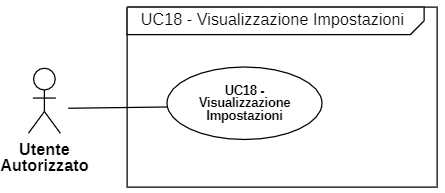
\includegraphics[scale=0.80]{images/UC13.png} 
		\caption{Descrizione grafica caso d'uso UC13}
	 \end{figure}

	\item \textbf{Attori}
	\begin{itemize} 
		\item \textit{Primari}: Utente autorizzato
		\item \textit{Secondari}: Non presenti
	\end{itemize}
	\item \textbf{Descrizione}: L'utente richiede la visualizzazione delle impostazioni.
	\item \textbf{Precondizione}: L'utente ha effettuato il login e si trova nella chat.
	\item \textbf{Postcondizione}: L'utente visualizza le impostazioni dell'applicazione.
	\item \textbf{Scenario principale}: \begin{enumerate}
		\item Utente interagisce con specifico pulsante per mostrare impostazioni;
		\item Utente visualizza le impostazioni.
	\end{enumerate}
\end{itemize}
\newpage